\chapter{Représentation de l’architecture globale}
\thispagestyle{EIP}

\section{Schématisation}
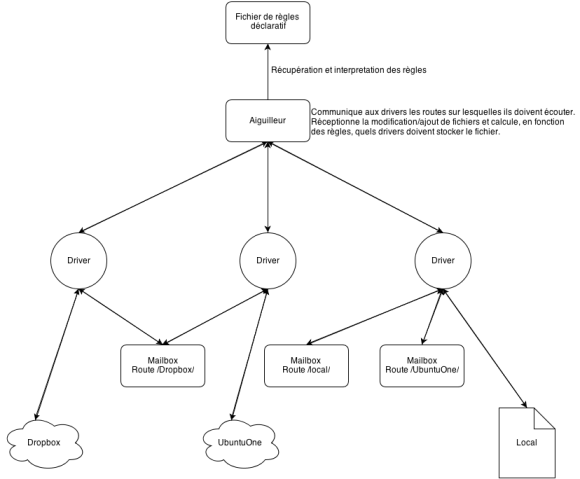
\includegraphics{schema_architecture_globale.png} 

\newpage
\section{Fichier de règles}

Le fichier de règles permet à l'utilisateur de configurer les choses suivantes:
\newline

\begin{itemize}
\itemsep1pt\parskip0pt\parsep0pt
\item
  Le nombre de répliques d'un fichier/dossier (À combien d'endroits il doit être stocké).
\item
  L'endroit où un fichier doit obligatoirement être stocké.
\item
  L'endroit où un fichier ne doit pas être stocké.
\newline
\end{itemize}

La définition de ces règles par l'utilisateur est facultative, Onitu a une configuration de base, completée et/ou modifiée par ce fichier.


\section{L'aiguilleur}
L'aiguilleur interpréte ce fichier, c'est lui qui donne l'ordre à un \emph{driver} d'écouter ou de ne plus écouter sur une route.
Il va également recevoir des messages de \emph{drivers} lui indiquant la création/suppression/mise à jour de certains fichiers, son rôle dans ce cas est d'informer les \emph{drivers} concernés de ce qu'ils doivent faire (écouter sur une nouvelle route par exemple).


\section{Les drivers}
Le rôle d'un \emph{driver} est d'assurer le CRUD (Create, Read, Update, Delete) des fichiers sur la plateforme de stockage qui lui est destinée (Local/UbuntuOne/Dropox etc).
C'est les \emph{drivers} qui réalisent la liaison entre Onitu et les différents services de stockage.


\section{Gestion de la communication entre les modules}
La communication entre les différents composants (\emph{drivers/aiguilleur}) se fera à l'aide d'un système de message fiable et rapide appelé ZeroMQ. Ce sont les \emph{mailbox} représentées sur le shéma qui contiendront ces messages.
